\section{\\Database Schema}~\label{sec:db-schema}

\begin{figure*}[h]
\centering
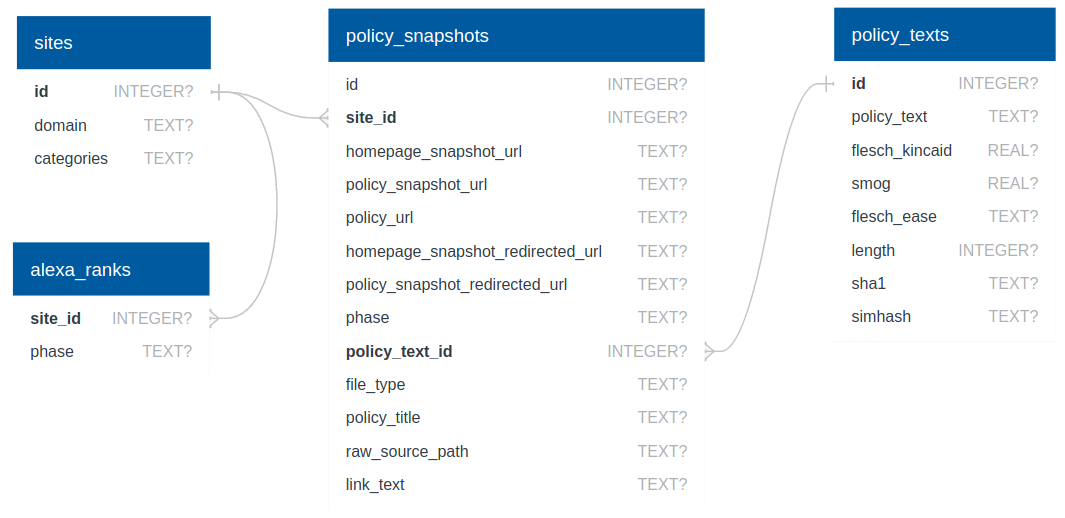
\includegraphics[width=0.8\textwidth]{figures/policy_db_schema.png}
\caption{The database schema.\gnote{Some column names are missing in this figure.}}
\label{fig:db_schema}
\end{figure*}

We combined policy text and metadata in an sqlite database with four tables: 
sites, alexa\_ranks, policy\_snapshots and policy\_texts.

\begin{description}
\item~\textbf{sites}: holds the website address and WebShrinker categories~\cite{Webshrinker}.
\item~\textbf{alexa\_ranks}: keeps the historical Alexa ranks for each site-interval pairs.
\item~\textbf{policy\_snapshots}: Policy snapshot URLs and associated metadata including year, phase (A, B, for first and the second six-month intervals, respectively), file\_type and     policy\_title.
%policy\_snapshots table contains two foreign keys: 1) ~\emph{policy\_text\_id} that points to the ID in the~\emph{policy\_texts} table and 2)~\emph{site\_id} that points to the ID in the~\emph{sites} table.
\item~\textbf{policy\_texts}: Contains extracted policy texts and text-based metadata such as length and readability scores.

\end{description}